\documentclass[tikz,border=6pt]{standalone}
\usepackage{tikz}
\begin{document}
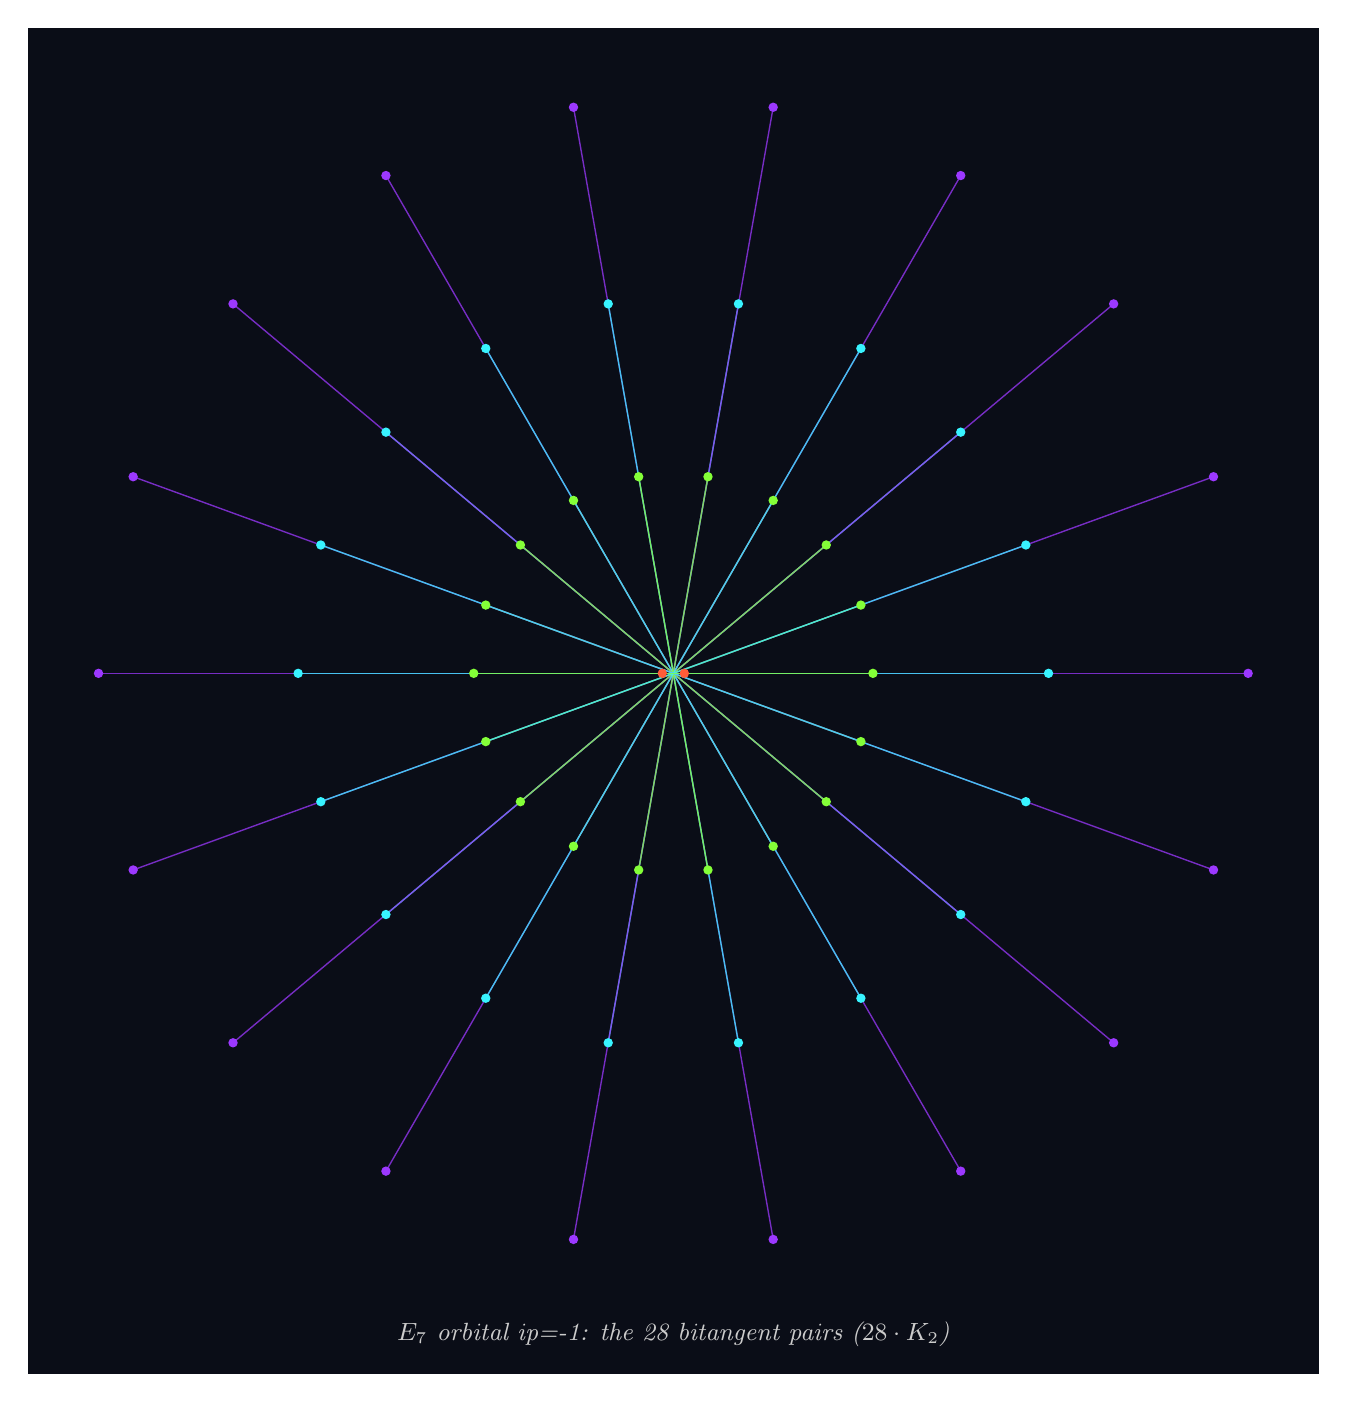
\begin{tikzpicture}
\definecolor{ring0}{rgb}{1.000,0.360,0.220}
\definecolor{ring1}{rgb}{0.516,1.000,0.220}
\definecolor{ring2}{rgb}{0.220,0.953,1.000}
\definecolor{ring3}{rgb}{0.610,0.220,1.000}
\definecolor{bg}{rgb}{0.04,0.05,0.09}
\fill[bg] (-8.2,-8.9) rectangle (8.2,8.2);
\draw[ring1,line width=0.5pt,opacity=0.75] (1.268,2.196)--(-1.268,-2.196);
\draw[ring3,line width=0.5pt,opacity=0.75] (-1.268,7.189)--(1.268,-7.189);
\draw[ring2,line width=0.5pt,opacity=0.75] (-0.827,4.692)--(0.827,-4.692);
\draw[ring2,line width=0.5pt,opacity=0.75] (0.827,4.692)--(-0.827,-4.692);
\draw[ring1,line width=0.5pt,opacity=0.75] (-1.268,2.196)--(1.268,-2.196);
\draw[ring3,line width=0.5pt,opacity=0.75] (1.268,7.189)--(-1.268,-7.189);
\draw[ring3,line width=0.5pt,opacity=0.75] (-3.650,6.322)--(3.650,-6.322);
\draw[ring2,line width=0.5pt,opacity=0.75] (3.650,3.063)--(-3.650,-3.063);
\draw[ring2,line width=0.5pt,opacity=0.75] (-3.650,3.063)--(3.650,-3.063);
\draw[ring3,line width=0.5pt,opacity=0.75] (3.650,6.322)--(-3.650,-6.322);
\draw[ring3,line width=0.5pt,opacity=0.75] (-5.592,4.692)--(5.592,-4.692);
\draw[ring3,line width=0.5pt,opacity=0.75] (5.592,4.692)--(-5.592,-4.692);
\draw[ring3,line width=0.5pt,opacity=0.75] (-6.860,-2.497)--(6.860,2.497);
\draw[ring1,line width=0.5pt,opacity=0.75] (2.382,-0.867)--(-2.382,0.867);
\draw[ring2,line width=0.5pt,opacity=0.75] (2.382,-4.126)--(-2.382,4.126);
\draw[ring1,line width=0.5pt,opacity=0.75] (0.440,-2.497)--(-0.440,2.497);
\draw[ring0,line width=0.5pt,opacity=0.75] (0.000,0.000)--(-0.000,-0.000);
\draw[ring1,line width=0.5pt,opacity=0.75] (-1.942,1.630)--(1.942,-1.630);
\draw[ring1,line width=0.5pt,opacity=0.75] (-1.942,-1.630)--(1.942,1.630);
\draw[ring3,line width=0.5pt,opacity=0.75] (7.300,-0.000)--(-7.300,0.000);
\draw[ring1,line width=0.5pt,opacity=0.75] (-0.440,-2.497)--(0.440,2.497);
\draw[ring1,line width=0.5pt,opacity=0.75] (-2.382,-0.867)--(2.382,0.867);
\draw[ring2,line width=0.5pt,opacity=0.75] (-2.382,-4.126)--(2.382,4.126);
\draw[ring3,line width=0.5pt,opacity=0.75] (6.860,-2.497)--(-6.860,2.497);
\draw[ring2,line width=0.5pt,opacity=0.75] (-4.765,0.000)--(4.765,-0.000);
\draw[ring2,line width=0.5pt,opacity=0.75] (4.477,1.630)--(-4.477,-1.630);
\draw[ring2,line width=0.5pt,opacity=0.75] (4.477,-1.630)--(-4.477,1.630);
\draw[ring1,line width=0.5pt,opacity=0.75] (2.535,-0.000)--(-2.535,0.000);
\fill[ring1] (1.268,2.196) circle (1.7pt);
\fill[ring3] (-1.268,7.189) circle (1.7pt);
\fill[ring2] (-0.827,4.692) circle (1.7pt);
\fill[ring2] (0.827,4.692) circle (1.7pt);
\fill[ring1] (-1.268,2.196) circle (1.7pt);
\fill[ring3] (1.268,7.189) circle (1.7pt);
\fill[ring3] (-3.650,6.322) circle (1.7pt);
\fill[ring2] (3.650,3.063) circle (1.7pt);
\fill[ring2] (-3.650,3.063) circle (1.7pt);
\fill[ring3] (3.650,6.322) circle (1.7pt);
\fill[ring3] (-5.592,4.692) circle (1.7pt);
\fill[ring3] (5.592,4.692) circle (1.7pt);
\fill[ring3] (1.268,-7.189) circle (1.7pt);
\fill[ring1] (-1.268,-2.196) circle (1.7pt);
\fill[ring2] (-0.827,-4.692) circle (1.7pt);
\fill[ring2] (0.827,-4.692) circle (1.7pt);
\fill[ring3] (-1.268,-7.189) circle (1.7pt);
\fill[ring1] (1.268,-2.196) circle (1.7pt);
\fill[ring2] (-3.650,-3.063) circle (1.7pt);
\fill[ring3] (3.650,-6.322) circle (1.7pt);
\fill[ring3] (-3.650,-6.322) circle (1.7pt);
\fill[ring2] (3.650,-3.063) circle (1.7pt);
\fill[ring3] (-5.592,-4.692) circle (1.7pt);
\fill[ring3] (5.592,-4.692) circle (1.7pt);
\fill[ring3] (-6.860,-2.497) circle (1.7pt);
\fill[ring1] (2.382,-0.867) circle (1.7pt);
\fill[ring2] (2.382,-4.126) circle (1.7pt);
\fill[ring1] (0.440,-2.497) circle (1.7pt);
\fill[ring0] (0.140,0.000) circle (1.7pt);
\fill[ring1] (-1.942,1.630) circle (1.7pt);
\fill[ring1] (-1.942,-1.630) circle (1.7pt);
\fill[ring3] (7.300,-0.000) circle (1.7pt);
\fill[ring1] (-0.440,-2.497) circle (1.7pt);
\fill[ring1] (-2.382,-0.867) circle (1.7pt);
\fill[ring2] (-2.382,-4.126) circle (1.7pt);
\fill[ring3] (6.860,-2.497) circle (1.7pt);
\fill[ring2] (-4.765,0.000) circle (1.7pt);
\fill[ring2] (4.477,1.630) circle (1.7pt);
\fill[ring2] (4.477,-1.630) circle (1.7pt);
\fill[ring1] (2.535,-0.000) circle (1.7pt);
\fill[ring1] (-2.535,0.000) circle (1.7pt);
\fill[ring2] (-4.477,1.630) circle (1.7pt);
\fill[ring2] (-4.477,-1.630) circle (1.7pt);
\fill[ring2] (4.765,-0.000) circle (1.7pt);
\fill[ring3] (-6.860,2.497) circle (1.7pt);
\fill[ring2] (2.382,4.126) circle (1.7pt);
\fill[ring1] (2.382,0.867) circle (1.7pt);
\fill[ring1] (0.440,2.497) circle (1.7pt);
\fill[ring3] (-7.300,0.000) circle (1.7pt);
\fill[ring1] (1.942,1.630) circle (1.7pt);
\fill[ring1] (1.942,-1.630) circle (1.7pt);
\fill[ring0] (-0.140,-0.000) circle (1.7pt);
\fill[ring1] (-0.440,2.497) circle (1.7pt);
\fill[ring2] (-2.382,4.126) circle (1.7pt);
\fill[ring1] (-2.382,0.867) circle (1.7pt);
\fill[ring3] (6.860,2.497) circle (1.7pt);
\node[white!80!black,font=\small\itshape] at (0,-8.4) {$E_7$ orbital ip=-1: the 28 bitangent pairs ($28\cdot K_2$)};
\end{tikzpicture}
\end{document}